\chapter{Outlook}
\label{chap:current}
\todo{end???}
The model diagnostic workflow proposed in the previous chapter has so far only been tested with binary input features.
This poses the question on how to expand to general numeric features.
While it is possible to adapt the used explanation algorithm to accept arbitrary features the resulting explanations are less interpretable.

\begin{figure}[t]
\centering
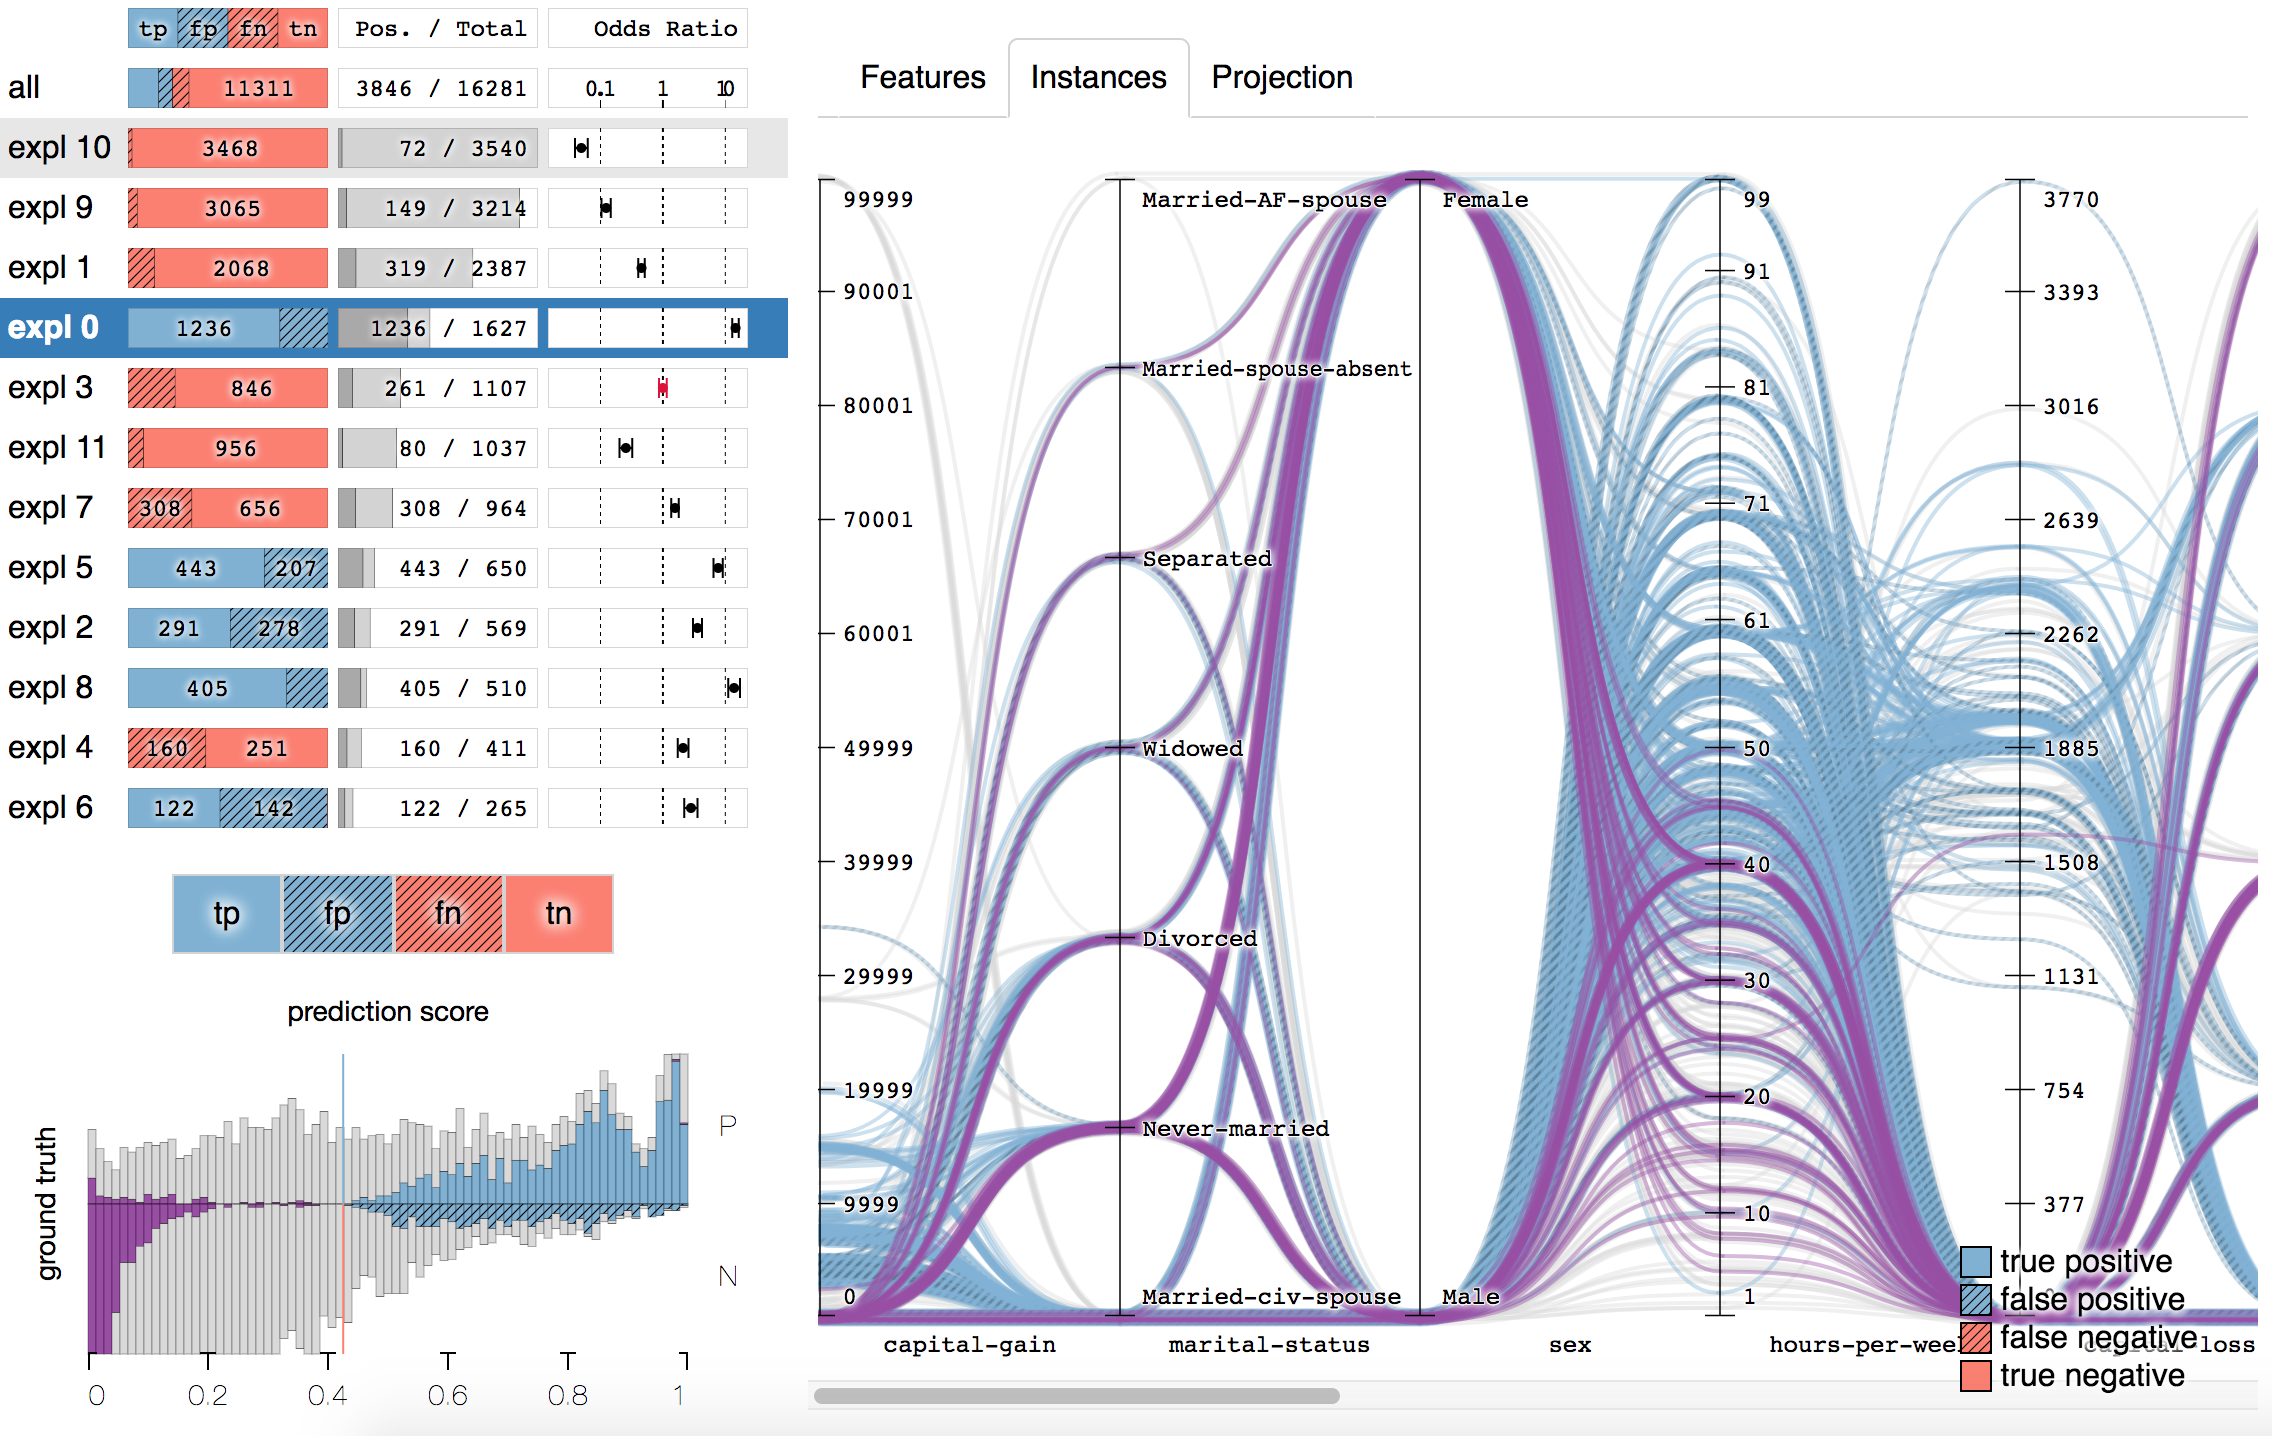
\includegraphics[height=16em]{figs/new_parallel.png}
\caption{
The extended interface to allow for non-binary data.
The list on the left shows the discovered ``decision sets".
Below that the distribution of prediction scores are shown.
A parallel coordinate view shows the instances covered by such a decision set (``expl 8") allowing non-binary input data.
The user highlights ``expl 10" showing its instances in purple.
}
\vspace*{-1em}
\label{figs:new_parallel}
\end{figure}
\begin{figure}
\centering
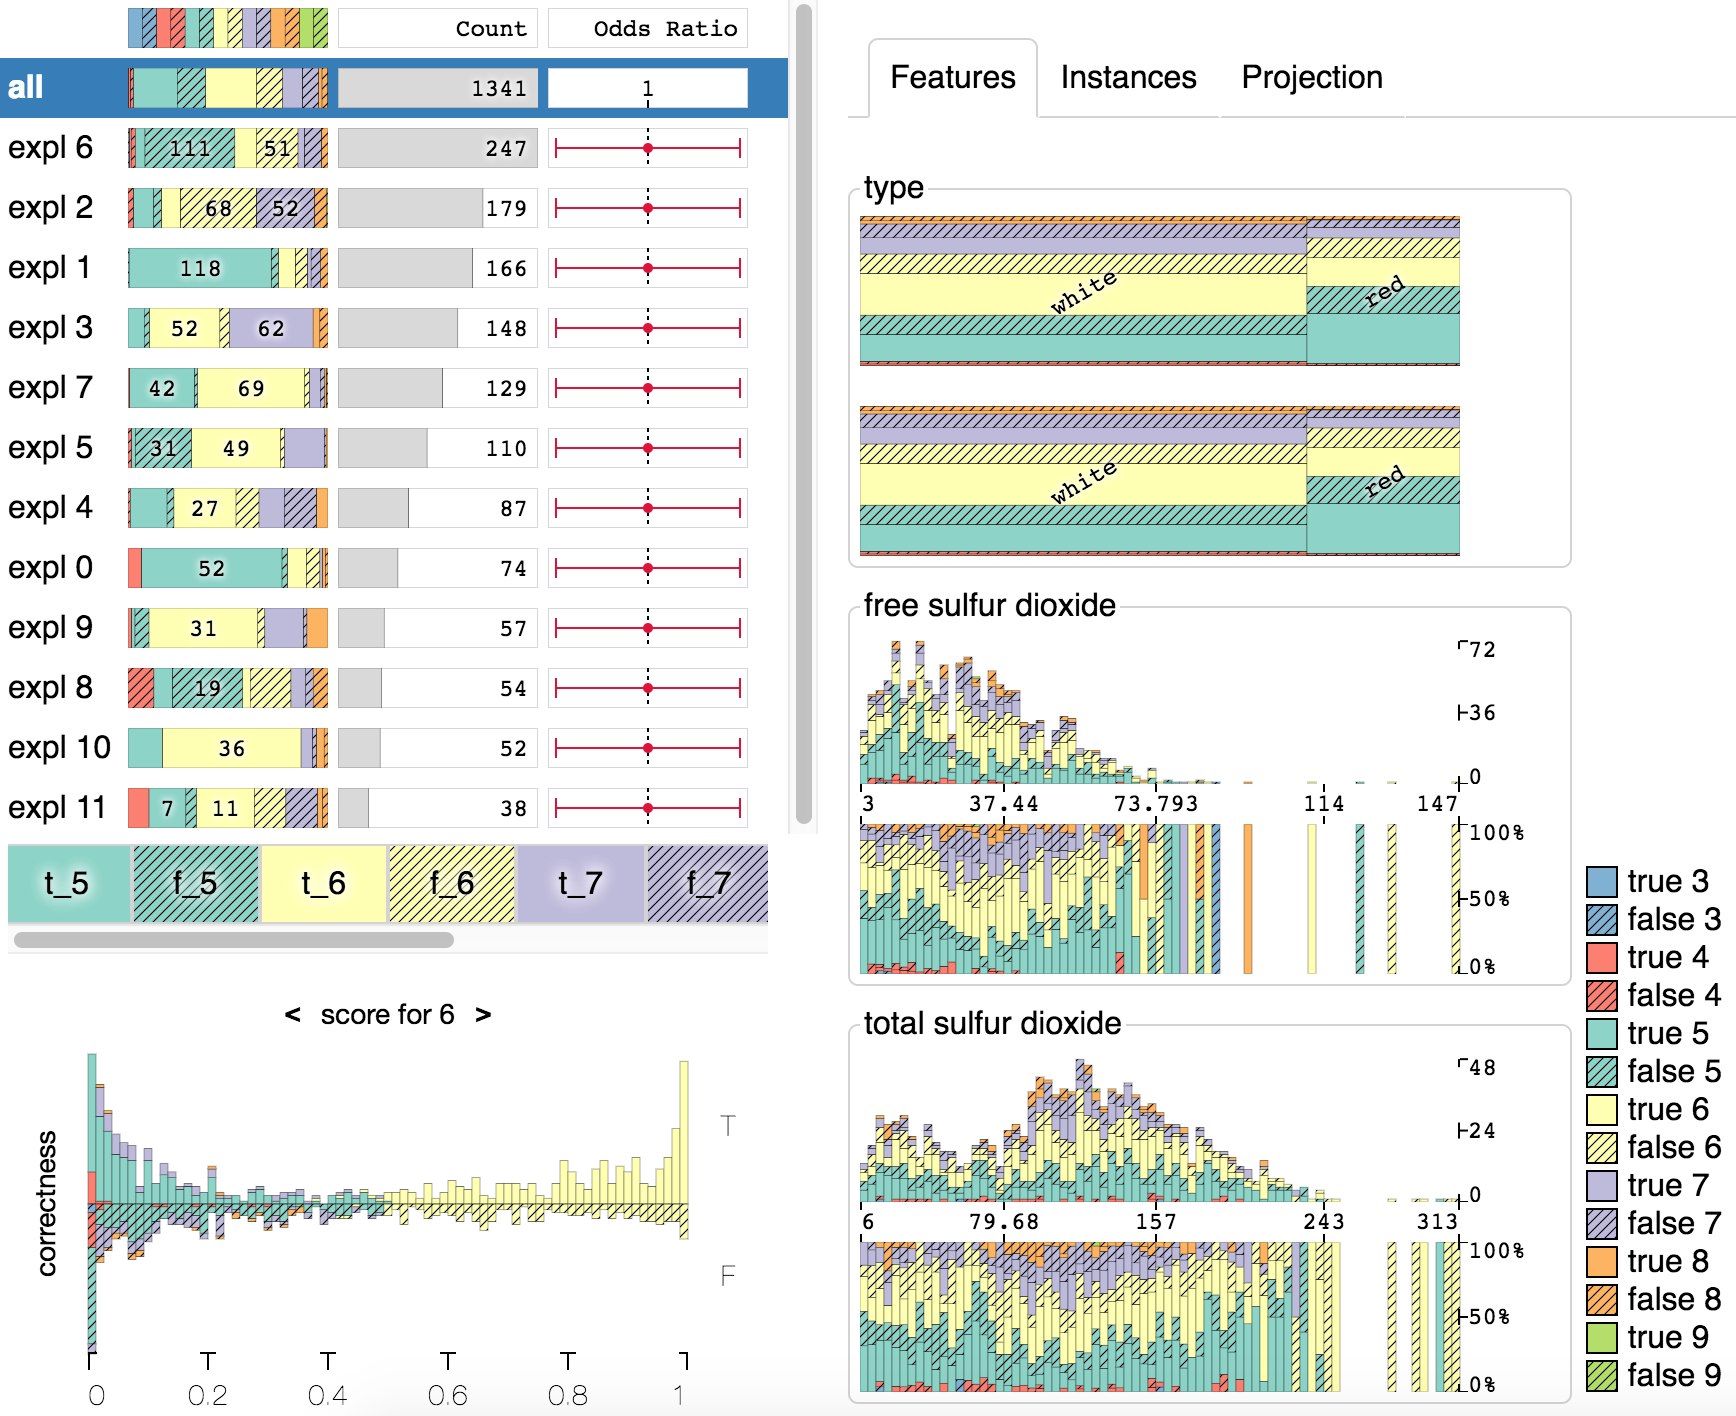
\includegraphics[height=16em]{figs/new_multiclass.png}
\caption{
The extended design even allows for multi-class classification tasks.
The left shows the different ``decision sets" and how the prediction scores for a given class are distributed.
On the right the distribution of classes per feature are shown.
}
\label{figs:new_multiclass}
\end{figure}

\section{Extending the Model Diagnostic Workflow}
In the case of binary features just naming the feature is enough to show its significance and how it is used by the machine learning model.
For numeric features additional information is needed.
For example, an explanation would be ``Feature A has high values" which poses further questions of the granularity of the description (``Feature A $>$ 5", ``Feature A $>$ average").
This introduces ambiguity and vagueness to the explanation.
A possible solution to this is to describe the explanation \emph{implicitly} by showing the distribution of values within features and how features interconnect.
The techniques proposed by \cite{seekaview} provide solutions to explore those relations effectively.

Another problem arising from generalizing the model diagnostic workflow is the observation that explanation algorithms include more features when the features are numerical (\ie, more features are relevant to the prediction).
The LIME algorithm \cite{DBLP:journals/corr/RibeiroSG16}, which produces feature weights for each instance, overcomes this issue by arbitrarily restricting features to a pre-chosen quantity (\eg, 10 features) by descending importance.
This restriction is independent of the actual distribution of feature weights.
It can happen that important features get removed or relatively unimportant features get included in the explanation.

\begin{figure}
\centering
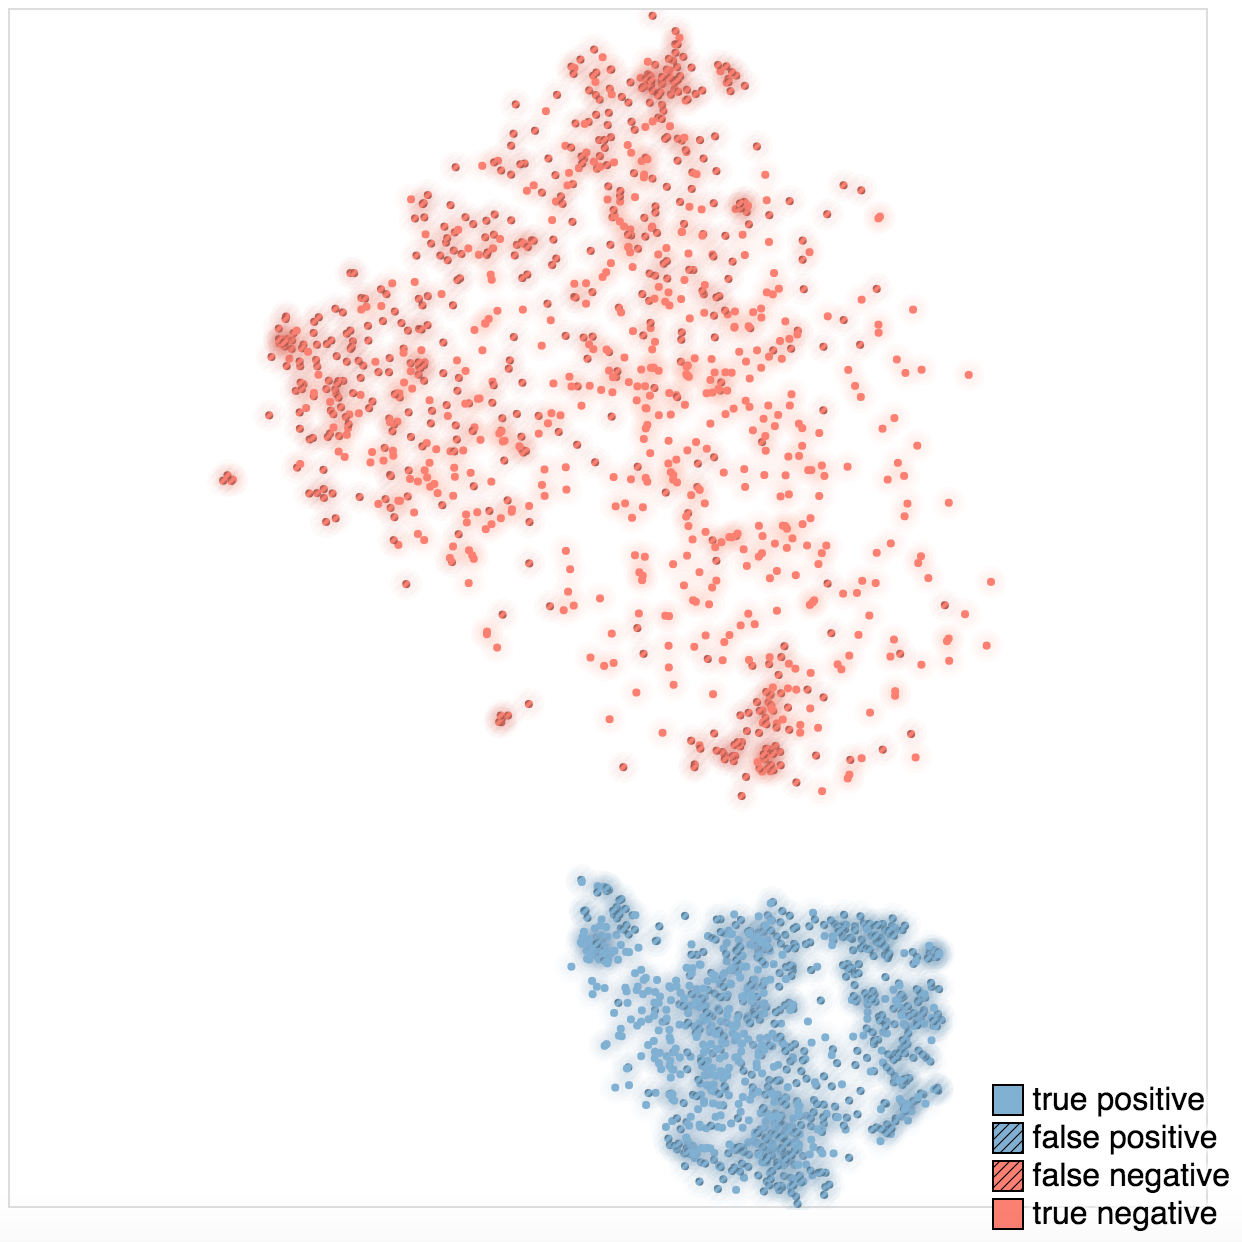
\includegraphics[height=22em]{figs/new_projection.png}
\caption{
Showing the distribution of instances according to the similarity of their explanations. The predicted label is also taken into account to allow for a clear separation of the two groups.
}
\label{figs:new_projection}
\end{figure}

With the above mentioned shift away from \emph{explicitly} describing explanations through their features towards \emph{implicitly} describing explanations through their instances, less care has to be taken to keep the number of relevant features in a range that is interpretable.
This opens up the aggregation of explanations from having explanations match exactly to being able to group together instances that are explained similarly.
This can be achieved by clustering the feature weights as obtained from the LIME algorithm which solves the problem of arbitrarily cutting off features from explanations as all features are included in the distance metric for clustering.
The resulting ``decision sets" can then be visualized (see Figures~\ref{figs:new_parallel}, \ref{figs:new_multiclass}, and \ref{figs:new_projection})
\vspace*{-0.5em}

\section{Formal Evaluation}
The model diagnostic workflow proposed in \chapref{chap:explainer} has not been formally evaluated.
We obtained information about its effectiveness through evidence from its use to improve machine learning models.
However, this does not guarantee that using explanations for machine learning models actually have a positive impact on the human perception of the quality of a model.
We are planning to run a study that aims to determine how the model diagnostic workflow changes the perceived trust and confidence in a model.
Besides subjectively measuring trust and confidence we are presenting decisions made by a model alongside information about their underlying data and asking participants to decide whether the decision is correct.
In one condition the participant has been exposed to only basic statistical performance measures of the machine learning models.
In the other condition the participant has the opportunity to use an implementation of our model diagnostic workflow to gain deeper understanding into the strengths and weaknesses of the model.
We have not started to run the study yet.

% The work shown so far provides an overview of how and where explanations of
% machine learning models can be helpful.
% However, it also shows gaps and challenges that provide much opportunity for further
% research.
% Especially for output only explanation there is still much room for improvements.
% Also, related research for interaction explanations
% (\cite{DBLP:journals/corr/RibeiroSG16} and \cite{Martens:2014:EDD:2600518.2600523})
% show a spectrum of different strategies on how to create those explanations but
% also show that there is still a lack of effective visual analytics tools conveying
% those explanations in a human understandable form.
% Two current projects address those challenges.

% \begin{figure}[b!]
\centering
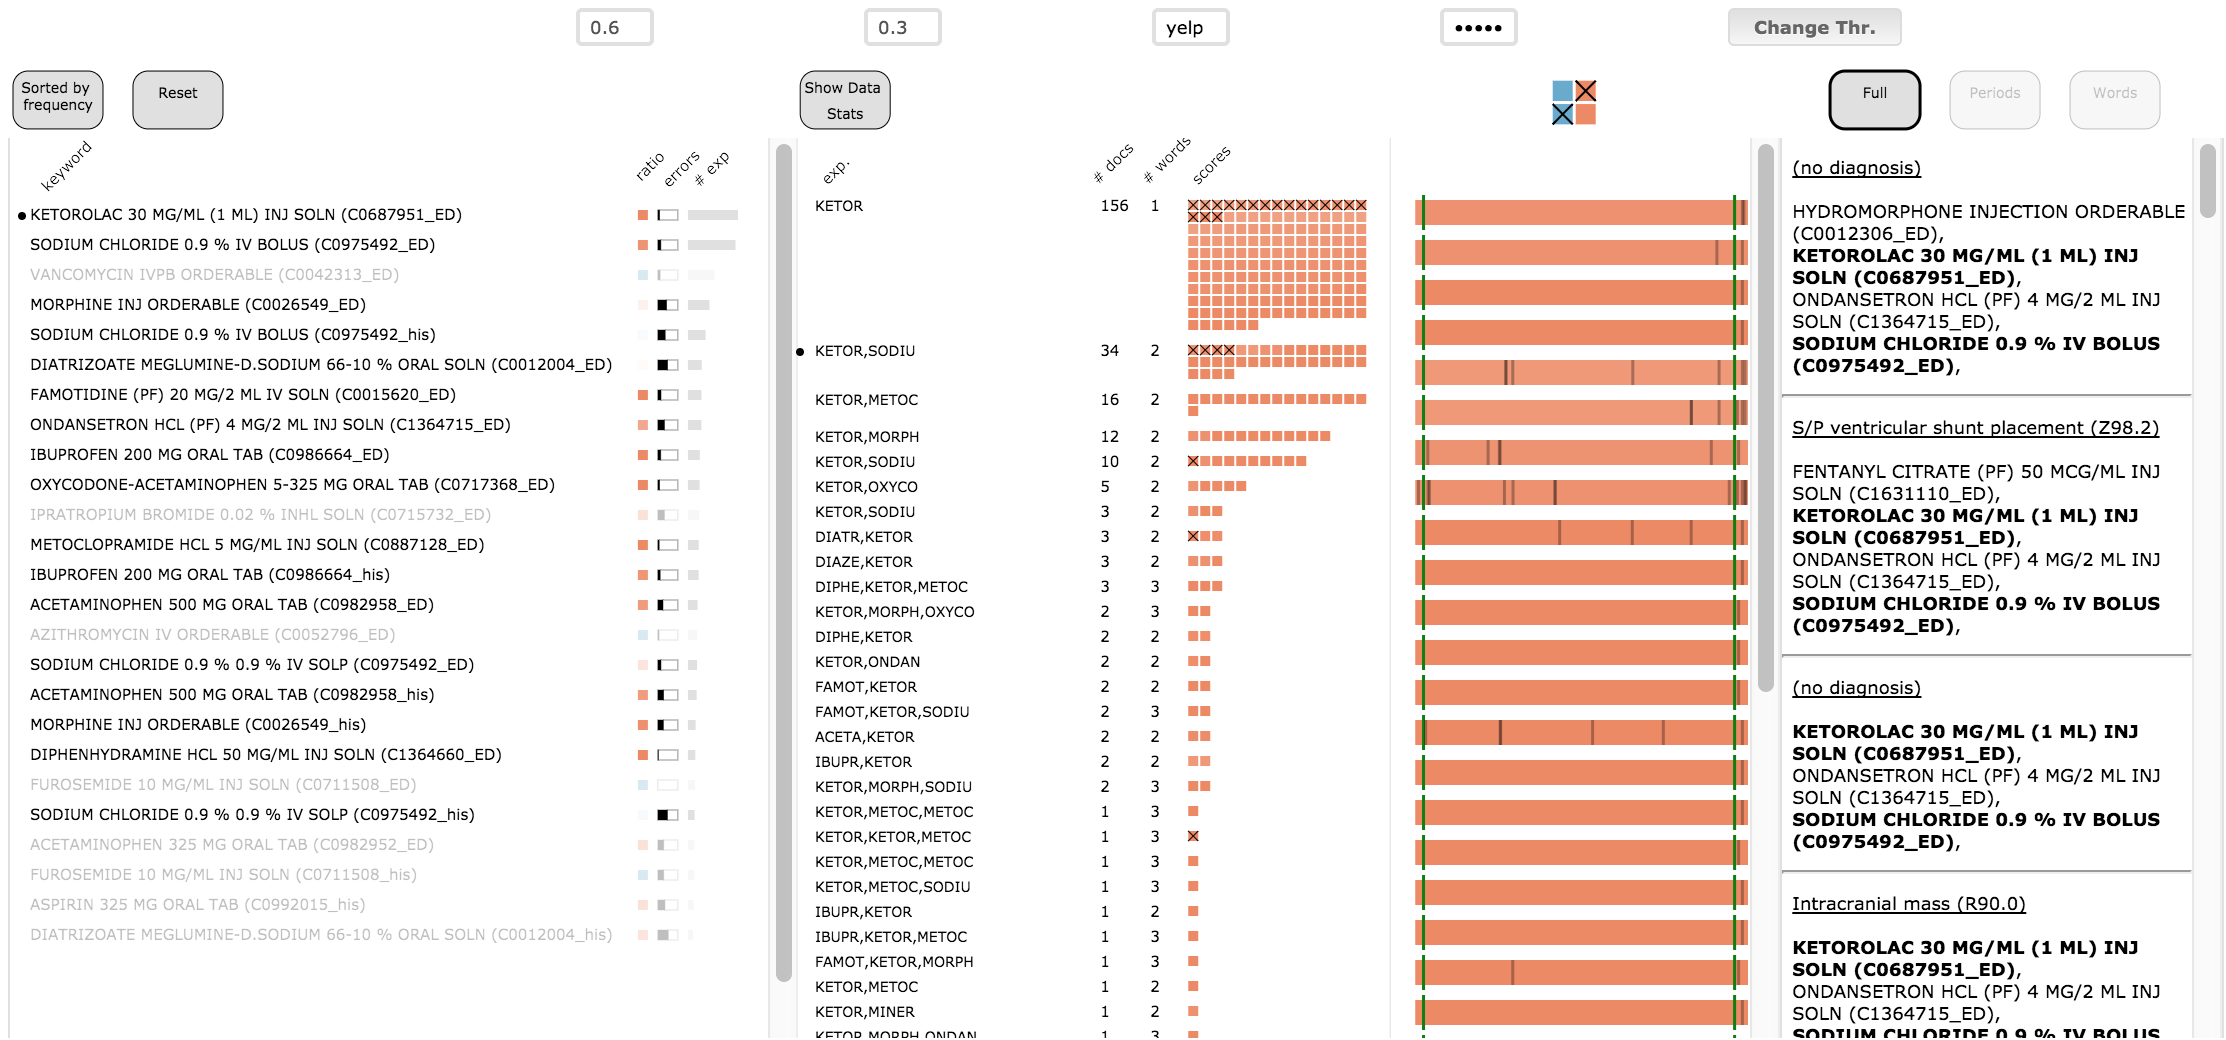
\includegraphics[width=0.8\linewidth]{figs/current/paolo_explain}
\caption{
Interface for exploring explanations for data points.
}
\label{figs:paolo_explain}
\end{figure}

% \section{Current Projects}
% The first project, in collaboration with Paolo Tamag, addresses the visual analytics
% aspect of providing an effective user interface to explore and understand machine
% generated interaction explanations.
% The interface, shown in \figref{figs:paolo_explain},
% leverages the explanation generation strategy developed by
% \cite{Martens:2014:EDD:2600518.2600523} for explaining predictions
% in text classification tasks.
% It offers explanation exploration to find data points with similar reasons
% for their predicted outcome.
% In the interface the list on the left shows the terms most commonly occurring in explanations.
% After selection explanations containing the selected terms are shown in the middle
% column.
% Information about falsely predicted data points are shown as well.
% Explanations can be further inspected by listing all matching data points (right).
% Terms from the explanation are highlighted.
% Further work needs to be done to utilize the interplay of data driven clusters
% and explanation driven clusters.

% The second project aims to improve output only explanations.
% Here, only prediction scores are used to generate explanations.
% In the current state of the project paths towards the highest scoring item
% are computed on existing data points.
% The resulting tree graph structure can then be explored and used for
% explanation generation.
% This technique helps analysts find and understand clusters of similarly behaving
% data points and regions of great prediction score fluctuation in the item space.
% Initial experiments of visual analytics approaches can be seen in
% \figref{figs:current_adj},
% \figref{figs:current_graph}, and
% \figref{figs:current_burst}.
% Further work needs to be done in terms of summarizing groupings and guidance to
% interesting areas in the item space.

% \begin{figure}[b!]
\centering
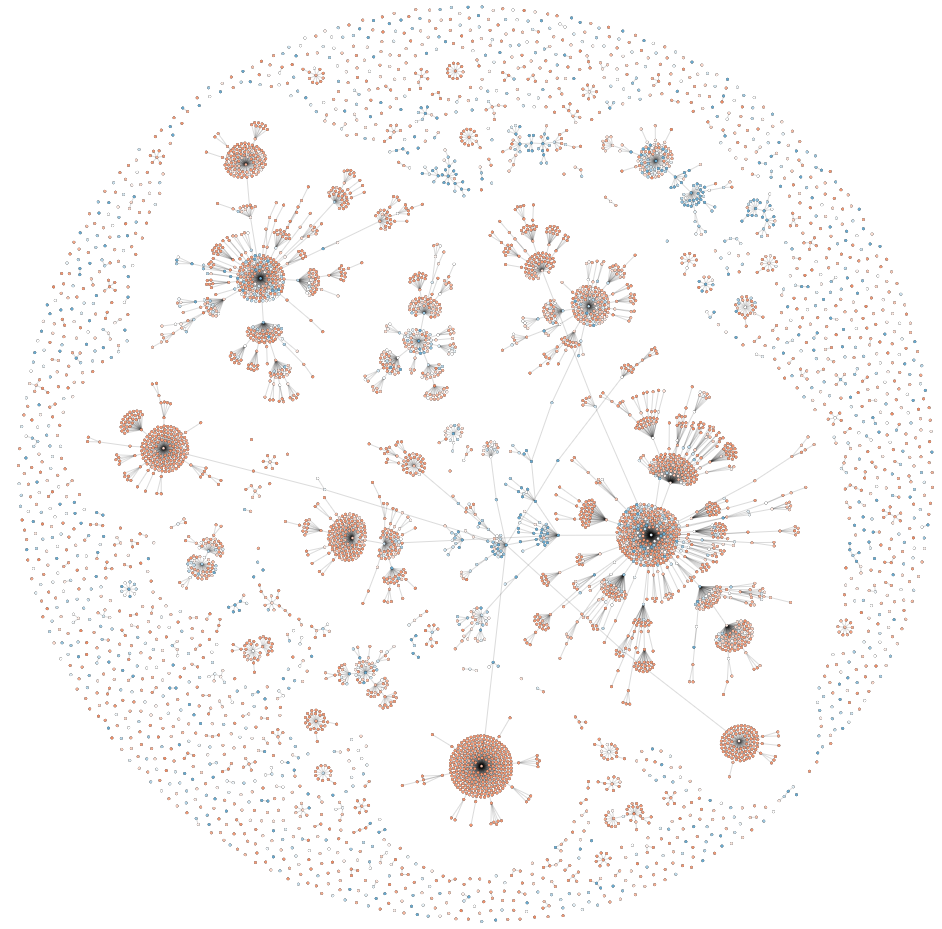
\includegraphics[width=0.5\linewidth]{figs/current/graph_d2}
\caption{
Node-link diagram showing how neighborhoods of data points are interconnected
with increasingly larger distances.
The edges of the directed graph always lead to points with a higher prediction score.
Especially of interest are label flips (ie., the prediction score increases by a wide
margin) or neighborhoods with consistent labels.
}
\label{figs:current_graph}
\end{figure}

% \begin{figure}
\centering
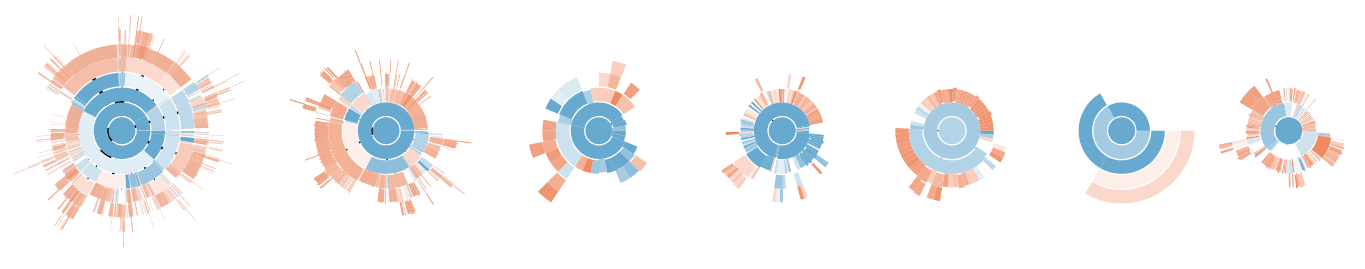
\includegraphics[width=\linewidth]{figs/current/burst_d2_top}
\caption{
Isolated neighborhoods shown as sunburst charts.
Each segment represents one data point.
The center indicates the data point with the highest score.
The distance to the center roughly corresponds with the number of changes
to the feature vector that are necessary to turn a point into the point at the center.
The size of the segments corresponds to the amount of points ``flowing"
through a point towards the center.
}
\label{figs:current_burst}
\end{figure}

% \begin{figure}
\centering
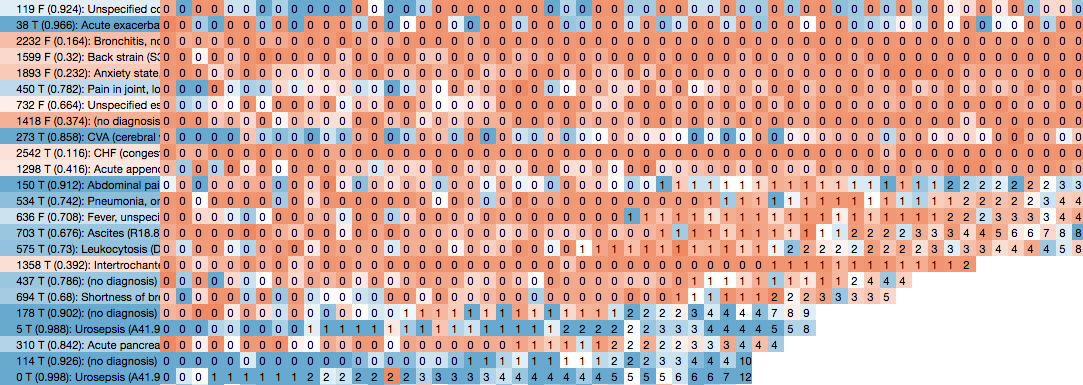
\includegraphics[width=\linewidth]{figs/current/adj_top}
\caption{
Neighborhoods of data points.
Each row represents one neighborhood with its representative (the point with the
highest prediction score) shown on the right.
Each cell represents one data point of the neighborhood.
The background color indicates the prediction score.
The numbers show how many changes in the feature vector are necessary to turn the
point into the representative.
}
\label{figs:current_adj}
\end{figure}

\chapter{Dissertation Outline and Progress}
\label{chap:thesis}
\section{Proposed Outline}
Below is the proposed outline of the planned dissertation, with references to previous research.

\begin{enumerate}[label*=\arabic*.]
    \item Introduction
    \begin{enumerate}[label*=\arabic*.]
        \item Machine Learning
        \begin{enumerate}[label*=\arabic*.]
            \item Predictive Modeling
            \item Popular Algorithms
        \end{enumerate}
        \item Motivation
        \item Related Work
        \item Use Case: Machine Learning for Health Care
    \end{enumerate}
    \item Feature Selection for Understanding Models
    \begin{enumerate}[label*=\arabic*.]
        \item INFUSE: Interactive Feature Selection for Predictive Modeling of High Dimensional Data (\textbf{publication}) ~\cite{infuse}
        \item Context
        \item Lessons Learned
    \end{enumerate}
    \item Partial Dependence for Understanding Models
    \begin{enumerate}[label*=\arabic*.]
        \item Prospector: Visual Inspection of Black-box Machine Learning Models (\textbf{publication}) ~\cite{prospector16}
        \item Context
        \item Lessons Learned
    \end{enumerate}
    \item Explanations for Understanding Models
    \begin{enumerate}[label*=\arabic*.]
        \item A Workflow for Visual Diagnostics of Binary Classifiers using Instance-Level Explanations (\textbf{publication}) ~\cite{explainer}
        \item Context
        \item Lessons Learned
    \end{enumerate}
    \item Generalization and Limitations of Explanations
    \begin{enumerate}[label*=\arabic*.]
        \item Generalization of Explanations to Non-Binary Data (\textbf{TBD})
        \item Study on Impacts of Explanations for Model Confidence and Trust (\textbf{TBD})
    \end{enumerate}
    \item Discussion
    \begin{enumerate}[label*=\arabic*.]
        \item Limitations and Assumptions of Black-Box Analysis
        \item Generalization to Other Forms of Machine Learning
        \item Implications
    \end{enumerate}
    \item Conclusion and Future Work
\end{enumerate}
\newpage
